
\section{System synthesis}
Figure \ref{img-web} shows the spider web that represents the way the variables are relating; the abbreviation CC, corresponds to cryptocurrencies. 

\begin{figure}[H]
	\centering
    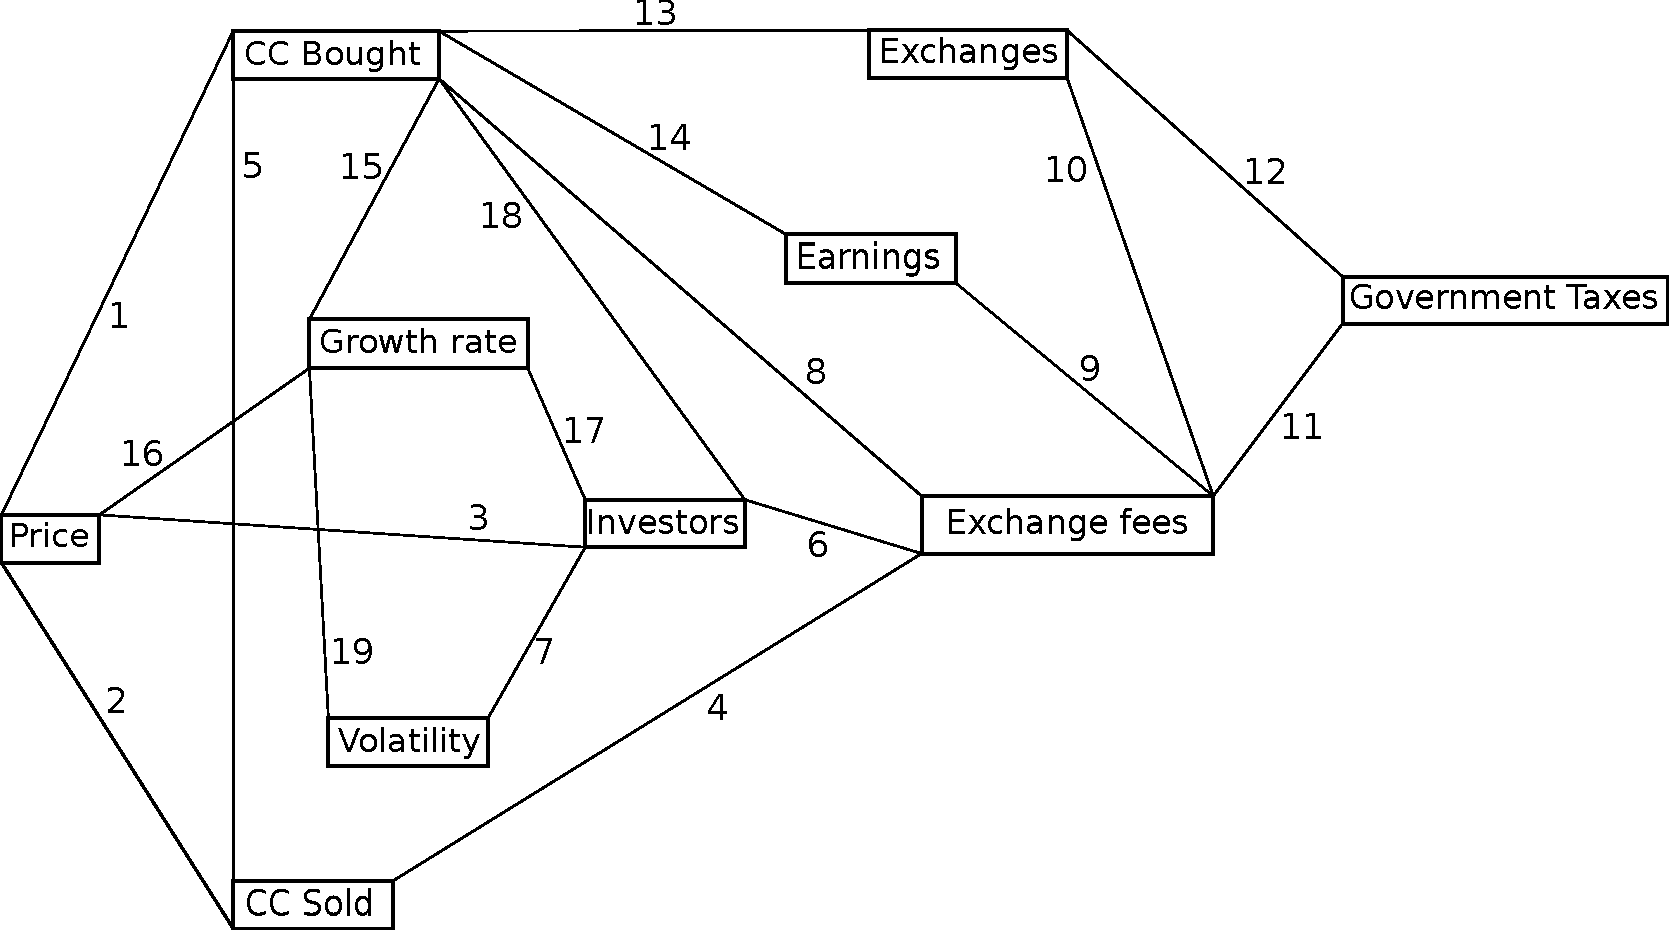
\includegraphics[scale=0.5]{files/SpiderWeb.pdf}
    \caption{SpiderWeb for the system described}
    \label{img-web}
\end{figure}

\noindent The numbers in the spider web represent the relationships between the variables, therefore it can be seen every relationship one by one.
For this analysis it is necessary to know as much as cryptocurrencies bought or sold, referenced to a specific cryptocurrency.
\begin{enumerate}
  \item Price of a cryptocurrency $\iif$ Cryptocurrencies bought: a simple directly proportional relationship, which is that the price depends on number of cryptocurrencies bought, for example if the people buy more of a cryptocurrency in specific, the price will increase. 
  \item Price of a cryptocurrency $\iif$ Cryptocurrencies sold: is a similar relation like the first one, because is also directly proportional; likewise, the number of the cryptocurrencies sold depends on the price.
  \item Price of a cryptocurrency $\iif$ Number of investors: this is a relation that consist in the price basically, is that to say that number of investors depends on the price of a cryptocurrency, so if the price of a cryptocurrency increase, the number of investors will increase as well.
  \item Cryptocurrencies sold $\iif$ Exchange fees: the taxes of the exchanges vary depends of the number of cryptocurrencies sold, because if the exchanges sold a lot of cryptocurrencies is not necessary to increase their taxes, but if the opposite happens they will need to augment their taxes.
  \item Cryptocurrencies sold $\iif$ Cryptocurrencies bought: this can clearly be seen and is that the number of cryptocurrencies sold depends in the number that been bought.
  \item Number of investors $\iif$ Exchange fees: a possible augment in the taxes of the exchanges, will decrease the number of investors, because they are not going to earn the same amount of money, accordingly the number of investors depends in the taxes of exchanges.  
  \item Volatility $\iif$ Number of investors: the relationship between these variables is inversely proportional, because as it increases the volatility, the number of investors decrease. 
  \item Exchange fees $\iif$ Cryptocurrencies bought: If the taxes of exchanges change, the number of cryptocurrencies bought will change.
  \item Exchange fees $\iif$ Earnings of investors: a decrease in the taxes of the exchanges, will produce an increase in the earnings of an investor, because they are going to pay less to the exchanges to change an specific cryptocurrency for regular money.  
  \item Number of exchanges $\iif$ Exchange fees: supposed an increase in the number of exchanges, this will generate a competition in the market between the exchanges, so to sell more they are going to reduce their taxes.
  \item Exchange fees $\iif$ Government taxes to exchanges: let us think in the taxes of the banks and the taxes of the government to the banks. What happened if the government augment their taxes? The answer to this question is very simple, if this happens the exchanges need to increase their taxes to cope that. The same thing happens with the taxes of exchanges and the government taxes. 
  \item Government taxes to exchanges $\iif$ Number of exchanges: if the taxes of the government are higher these in a lapse of time will generate a decrease in the number of exchanges because they are ``losing'' money paying to the government. 
  \item Number of exchanges $\iif$ Cryptocurrencies bought: in the case of the demand of  cryptocurrencies increase, this will generate a increase of the number of exchanges, to solve the bought of cryptocurrencies.
  \item Earnings $\iif$ Cryptocurrencies Bought: If consumers earn more, they can afford buying more.
  \item Growth rate $\iif$ Cryptocurrencies bought: If the growth rate increases, consumers will buy more of that cryptocurrency.
  \item Price $\iif$ Growth rate: A decrease in the price of a cryptocurrency implies that the growth rate reduces.
  \item Growth rate $\iif$ Investors: If the cryptocurrency is growing, human beings will invest more to get more profit.
  \item Investors $\iif$ Cryptocurrencies bought: If there are more investors, there will be more cryptocurrencies bought.
  \item Growth rate $\iif$ Volatility: Am augment in the growth rate will generate an increase in the volatility.
\end{enumerate}
Obviously, all the variables are important and it is necessary to see the relationships between them but is easy to see that one of the variables that more affect the system are the prices, both cryptocurrency and taxes of the exchanges and the government. It is important to highlight that the volatility affects the most of market, but anything affects it. Let us understand the volatility as the change of the market in an specific time, so it could be interpreted as the risk of making money on an investment, therefore if the volatility is  high then the probability of making money is high as well, but also the probability of losing money, because the market is changing constantly.
